%!TEX root = main.tex
In the following, we will assume that $\wdd = 3, \bdd = 2$. We will use the nodes-as-edges notation in the following since black nodes have degree 2.

\section{Known logarithmic problems}\label{sec:known}
\subsubsection{The 3-vertex coloring}
It is known that d-vertex coloring has a complexity $\Theta(\log_dn)$ on d-regular trees \cite{DBLP:journals/corr/ChangKP16}, therefore we can classify the 3-vertex coloring problem on 3-regular trees: $$W = \{AAA,BBB,CCC\}, B =\{AB,AC,BC\}$$

\subsubsection{The 3-edge coloring}
First, we know that d-edge coloring has a complexity $\mathcal{O}(\log_dn)$  on d-regular trees with $d\geq 3$ \cite{DBLP:journals/corr/abs-1708-04290}.
We also know that 3-edge coloring has a complexity $\Omega(\log_n)$ on 3-regular trees \cite{balliu2019locality}, we can then classify the 3-edge coloring problem on 3-regular trees: $$W = \{ABC\}, B=\{AA,BB,CC\}$$

\section{Logarithmic upper bounds}
\subsection{Logarithmic upper bound using sinkless and sourceless orientation}
We know that creating a sinkless and sourceless orientation (SSO) in a 3 regular tree has a $\Theta(\log(n))$ complexity \cite{1}. Let's use this result to show that some 3 labelling problems have a $\mathcal{O}(\log(n))$ complexity. For each problem, we will show that for any given graph with a SSO, a constant algorithm capable of solving it exists.\\
The SSO ensures that, on any 3 regular graph, a given node $u$ with a degree 3 has either:
\begin{itemize}
    \item 2 outgoing edges and 1 incoming edge
    \item 1 outgoing edge and 2 incoming edges
\end{itemize}
The former will be denoted $X$ when the latter $Y$
\subsubsection[(W = (ABC, BCC), B = (AC,BC)]{$W = \{ABC, BCC\}$, $B = \{AC, BC\}$}
\begin{itemize}
    \item We label the nodes of type $X$ with $BCC$ such that the port corresponding to the incoming edge is labelled with $B$
    \item We label the nodes of type $Y$ with $ABC$ such that the port corresponding to the outgoing edge is labelled with $C$
\end{itemize}

\subsubsection[(W = (AAC, BCC), B = (AC,BC)]{$W = \{AAC, BCC\}$, $B = \{AC, BC\}$}


\begin{itemize}
    \item We label the nodes of type $X$ with $BCC$ such that the port corresponding to the incoming edge is labelled with $B$
    \item We label the nodes of type $Y$ with $AAC$ such that the port corresponding to the outgoing edge is labelled with $C$
\end{itemize}

We can see that the respective white constraint of each problem is respected since every configuration used are in it. Also, any oriented edge $(u,v)$ starts from a port of $u$ labelled with a $C$ and can either end on a port of $v$ labelled with $A$ or $B$, since the black constraints contains both $AC$ and $BC$ in both of these cases the configuration are valid. Since this procedure takes 0 rounds, these problems have the same complexity as the SOO.



\subsection{Logarithmic upper bound using even orientation}
Again, we know that creating an even orientation (EO) in a 3 regular has a $\Theta(\log(n))$ complexity \cite{1}. Let's use this result to show that some 3 labelling problems have a $\mathcal{O}(\log(n))$ complexity. For each problem, we will show that for any given graph with a EO, a constant algorithm capable of solving it exists.\\
The EO ensures that, on any 3 regular graph, a given node $u$ with a degree 3 has either:
\begin{itemize}
    \item 2 outgoing edges and 1 incoming edge
    \item 0 outgoing edge and 3 incoming edges
\end{itemize}
The former will be denoted $X$ when the latter $Y$
\subsubsection[(W = (ABC, CCC), B = (AC,BC)]{$W = \{ABC, CCC\}$, $B = \{AC, BC\}$}
\begin{itemize}
    \item We label the nodes of type $X$ with $ABC$ such that the port corresponding to the incoming edge is labelled with $C$
    \item We label the nodes of type $Y$ with $CCC$
\end{itemize}

\subsubsection[(W = (X0X1X2, X3CC), B = (AC,BC)]{All the problems where : $W = \{X_0X_1X_2, X_3CC\}$, $B = \{AC, BC\}$ with $X_i \in \{A,B\}$ for $i=0,1,2,3$}
\begin{itemize}
    \item We label the nodes of type $X$ with $X_3CC$ such that the port corresponding to the incoming edge is labelled with $X_3$
    \item We label the nodes of type $Y$ with $X_0X_1X_2$
\end{itemize}
We can see that the respective white constraint of each problem is respected since every configuration used are in it. Also, any edge $(u,v)$ is always labelled either with $AC$ or $BC$,in both of these cases the configuration are valid. Since this procedure takes 0 rounds, these problems have the same complexity as the EO.


\subsection{Logarithmic upper bound using 3 vertex coloring and 3 edges coloring}
According to the section \ref{sec:known}, we know that both 3 vertex coloring and 3 edges coloring have a $\mathcal{O}(\log(n))$ complexity. Let's show that the 3 labelling problem $W = \{ABC\}, B = \{AC, AB, BC\}$ has as well a $\mathcal{O}(\log(n))$ complexity by describing an algorithm that solves it in time $\log(n)$\\\\
We start by producing a 3 edges coloring $\mathit{0,1,2}$ on the graph in time $\mathcal{O}(\log(n))$.
We also produce a 3 vertex coloring $\mathbf{0,1,2}$ in time $\mathcal{O}(\log(n))$\\\\
In the following, we denote the color of a node $u$ as $u_c$ and the color of an edge $e$ as $e_c$\\\\
We label the ports of a node $u$ in the following way:\\
For each port $p$ of $u$, let $e^p$ be the incident edge to $u$ corresponding to $p$. The algorithm labels $p$ with $$(u_c+e^p_c)\mod{3}$$.
\begin{table}
    \centering
    \begin{tabular}{r|ccc}
        \diagbox{$u_c$}{$e^p_c$} & $\mathit{0}$ & $\mathit{1}$ & $\mathit{2}$ \\
        \hline
        $\mathbf{0}$ & 0 & 1 & 2 \\
        $\mathbf{1}$ & 1 & 2 & 0 \\
        $\mathbf{2}$ & 2 & 0 & 1
        
    \end{tabular}
    \caption{Label of $p$ depending on $u_c$ and $e^p_c$}
    \label{tab:vertexedgecoloring}
\end{table}

The table \ref{tab:vertexedgecoloring} show all the possibilities. As we can see, on any given line of the table, there is always exactly 3 different labels, this implies that a given node must respect the white constraint $ABC$ given the output of the algorithm.

On the other hand, On any given column of the table, there is always exactly 3 different labels as well. This means that a given edge must always have its 2 incident nodes labelling their corresponding ports with different colors, it hence respect the black constraint $AB,AC,BC$

\subsection{The Rake and Compress Procedure}
\subsubsection{The concerned problems}
Using the rake and Compress Procedure we will show $\mathcal{O}(\log(n))$ on one problem and two classes of problems.
We write them below, note that for each of them $B=\{AB,CC\}$
\begin{itemize}
    \item $\Pi_0 = (3,2,W,B)$ where $W = \{ABC\}$
    \item The set of problem $S_1$ where $\Pi_1 = (3,2,W,B)\in S_1$ if and only if $W = \{ACC,BCX\}$\\where $X\in \{A,B,C\}$
    \item The set of problem $S_2$ where $\Pi_2 = (3,2,W,B)\in S_2$ if and only if $W = \{AAX,BCC\}$\\where $X \in \{A,B,C\}$
    \item The set of problem $S_3$ where $\Pi_3 = (3,2,W,B)\in S_3$ if and only if $W = \{AAX,BBC\}$\\where $X \in \{A,B,C\}$
\end{itemize}
\subsubsection{The Procedure}
We will present here a procedure that will be very useful to show $\mathcal{O}(\log(n))$ upper bounds. It is based on the Rake and compress procedure technique introduced by Miller and Reif \cite{RC} and the procedure RCP that emerged from it \cite{1}.

The idea here is to decompose the graph in multiple layers in a way that the number of layer is $L = \mathcal{O}(\log(n))$. We can then find an algorithm that iterates over the layers and labels every edges incident to nodes in it in time $O(1)$.

As a first step, for the sake of clarity, we redefine here the two definitions for the low-degree and the long path used in the procedure RCP \cite[p.21]{1}

We assume that we work on a tree Let $G = (V,E)$, with all the vertices properly colored, i.e. each vertex $u\in V$ is either colored in white, either colored in black.

\begin{defi} (low degree).
Let $w,b \in \{1,2\}$. We define that low-degree$(G,w,b)\subseteq V$ is the set of all white nodes having a degree at most $w$ and all black nodes having a degree at most $b$.
\end{defi}

\begin{defi} (long path).
Let $p \in \{1,2,...\}$. Let $X \subseteq V$ consists of all nodes of degree exactly 2. We define that long-paths$(G, p)\subseteq X$ consist of those nodes that belong to a connected component of size at least p in the sub-graph of G induced by X.
\end{defi}

The procedure $RCP(p)$ partitions the set of nodes $V$ into non-empty sets $V_1,V_2,...V_L$ for some $L = \mathcal{O}(\log(n))$ by iteration as follows \cite[p.23]{1}:
\begin{itemize}
    \item We start with $G_0 = G$
    \item From $G_i$ we create $V_{i+1} = $ low-degree$(G_i,1,1)\cup $ long-paths$(G_i,p)$
    \item $G_{i+1} = G_i- V_{i+1}$
\end{itemize}

By construction of such layers, when applying the procedure $RCP(p)$, each nodes must respect some properties. Indeed for $i \in \{1,2,...,L\}$ a node in a layer $V_i$ must be in one of the following:
\begin{itemize}
    \item low-degree $(G_{i-1},1,1)$.
    This induces that the node has at most 1 neighbor in a layer $V_j$ with $j \in \{i,i+1...,L\}$.
    
    \item long-paths $(G_{i-1},p)$.
    In this case the node can be in 2 different configuration :
    \begin{itemize}
        \item If it is an endpoint of the long path, it has one neighbor in $V_i$ and one neighbor in a layer $V_j$ with $j \in \{i,i+1...,L\}$ 
        \item If it is not an endpoint of the long path, it has two neighbors in $V_i$
    \end{itemize}
\end{itemize}
In all the cases, all its other neighbors must be in a layer $V_l$ with $l \in \{0,...,i-1\}$.

\subsubsection{The algorithm}

\begin{claim}\label{claim:path} 
\textit{It is possible to split a path of length $n\geq 11$ in at least 2 paths of consecutive nodes in time $\mathcal{O}(\log^*n)$ where each sub-path $P^i$ as a length $6\leq n_i \leq 28$ and 2 sub-paths can share at most 1 node. }
\begin{proof}
Let $P=(V,E)$ be the path.
\begin{itemize}
\item\textbf{Step 1 :} In constant time we "hide" the 5 nodes at the beginning of the path and the 5 at the end of it.
It then remains $n-10$ nodes, let's call this path $P_0=(V_0,E_0)$.\\
\item\textbf{Step 2 :} We run a first time the Maximal Independent Set algorithm on this $P_0$ nodes to produce the set $S_0\subseteq V_0$. This takes time $\mathcal{O}(\log^*n)$, and from that, we know that between 2 consecutive nodes in $S_0$ there can be between $2$ and $3$ edges.\\
\item\textbf{Step 3 :} We now crop the path by hiding nodes in order to have 2 nodes that are in $S_0$ as end point, this result in hiding between $0$ and $1$ node from each side of the path. The resulting path is denoted as $P_1=(V_1,E_1)$\\
\item\textbf{Step 4 :} We run again the Maximal Independent Set algorithm on $P_1$ where nodes that are not in $S_0$ are considered as edges to produce $S_1$, we know that between 2 consecutive nodes in $S_1$ there can be between $4$ and $9$ edges.\\
\item\textbf{Step 5 :} Again, we crop the path by hiding nodes in order to have 2 nodes that are in $S_1$ as end point, this result in hiding either $0$, $2$ or $3$ nodes from each side of the path. The resulting path is denoted as $P_2=(V_2,E_2)$\\
\item\textbf{Step 6 :} We run one last time the Maximal Independent Set algorithm on $P_2$ where nodes that are not in $S_1$ are considered as edges to produce $S_1$, we know that between 2 consecutive nodes in $S_2$ there can be between $8$ and $27$ edges.\\
\item\textbf{Step 7 :} Finally, we crop the path by hiding nodes in order to have 2 nodes that are in $S_2$ as end point, this result in hiding at most $9$ from each side of the path. The resulting path is denoted as $P_3=(V_3,E_3)$\\
\item\textbf{Step 8 :} We now define the sub-path endpoints as : 
\begin{itemize}
    \item The endpoints of the path
    \item The nodes in $S_2$.
\end{itemize}
\end{itemize}
First, let's show that there are at least 2 sub-path after this process, i.e, $|S_2|\geq 1$. Since there is at least 11 nodes in $P$, there must be at least 1 node in $P_0$ after hiding $10$ nodes. MIS will hence put at least 1 node in $S_0$, for the same reason, $|S_1|\geq 1$ and $|S_2|\geq 1$\\
Now :
\begin{itemize}
    \item If a sub-path $P^i$ is between an endpoint $u$ of the path and a node $v$ in $S_2$, we know that v must be at least at distance $6$ from $u$ since the nodes at a distance $\leq 4$ from $u$ where hidden during the process of selecting nodes for $S_2$. Hence, $6\leq n_i$. Also, in step 3, 5 and 7 we added respectively at most 1, 3 and 9 nodes to both of the 2 hidden nodes sets. Hence, $n_i \leq 5+1+3+9+1 = 19 \leq 28$
    \item If a sub-path $P^i$  is between two nodes $u$ and $v$ in $S_2$. As stated above, there are between $8$ and $27$ edges between 2 nodes in $S_2$ meaning between 9 and 28 nodes. Hence $6 \leq 9 \leq n_i \leq 28$

\end{itemize}
The figure \ref{fig:path} shows the running of the process.
\begin{figure}[htb]
    \centering
    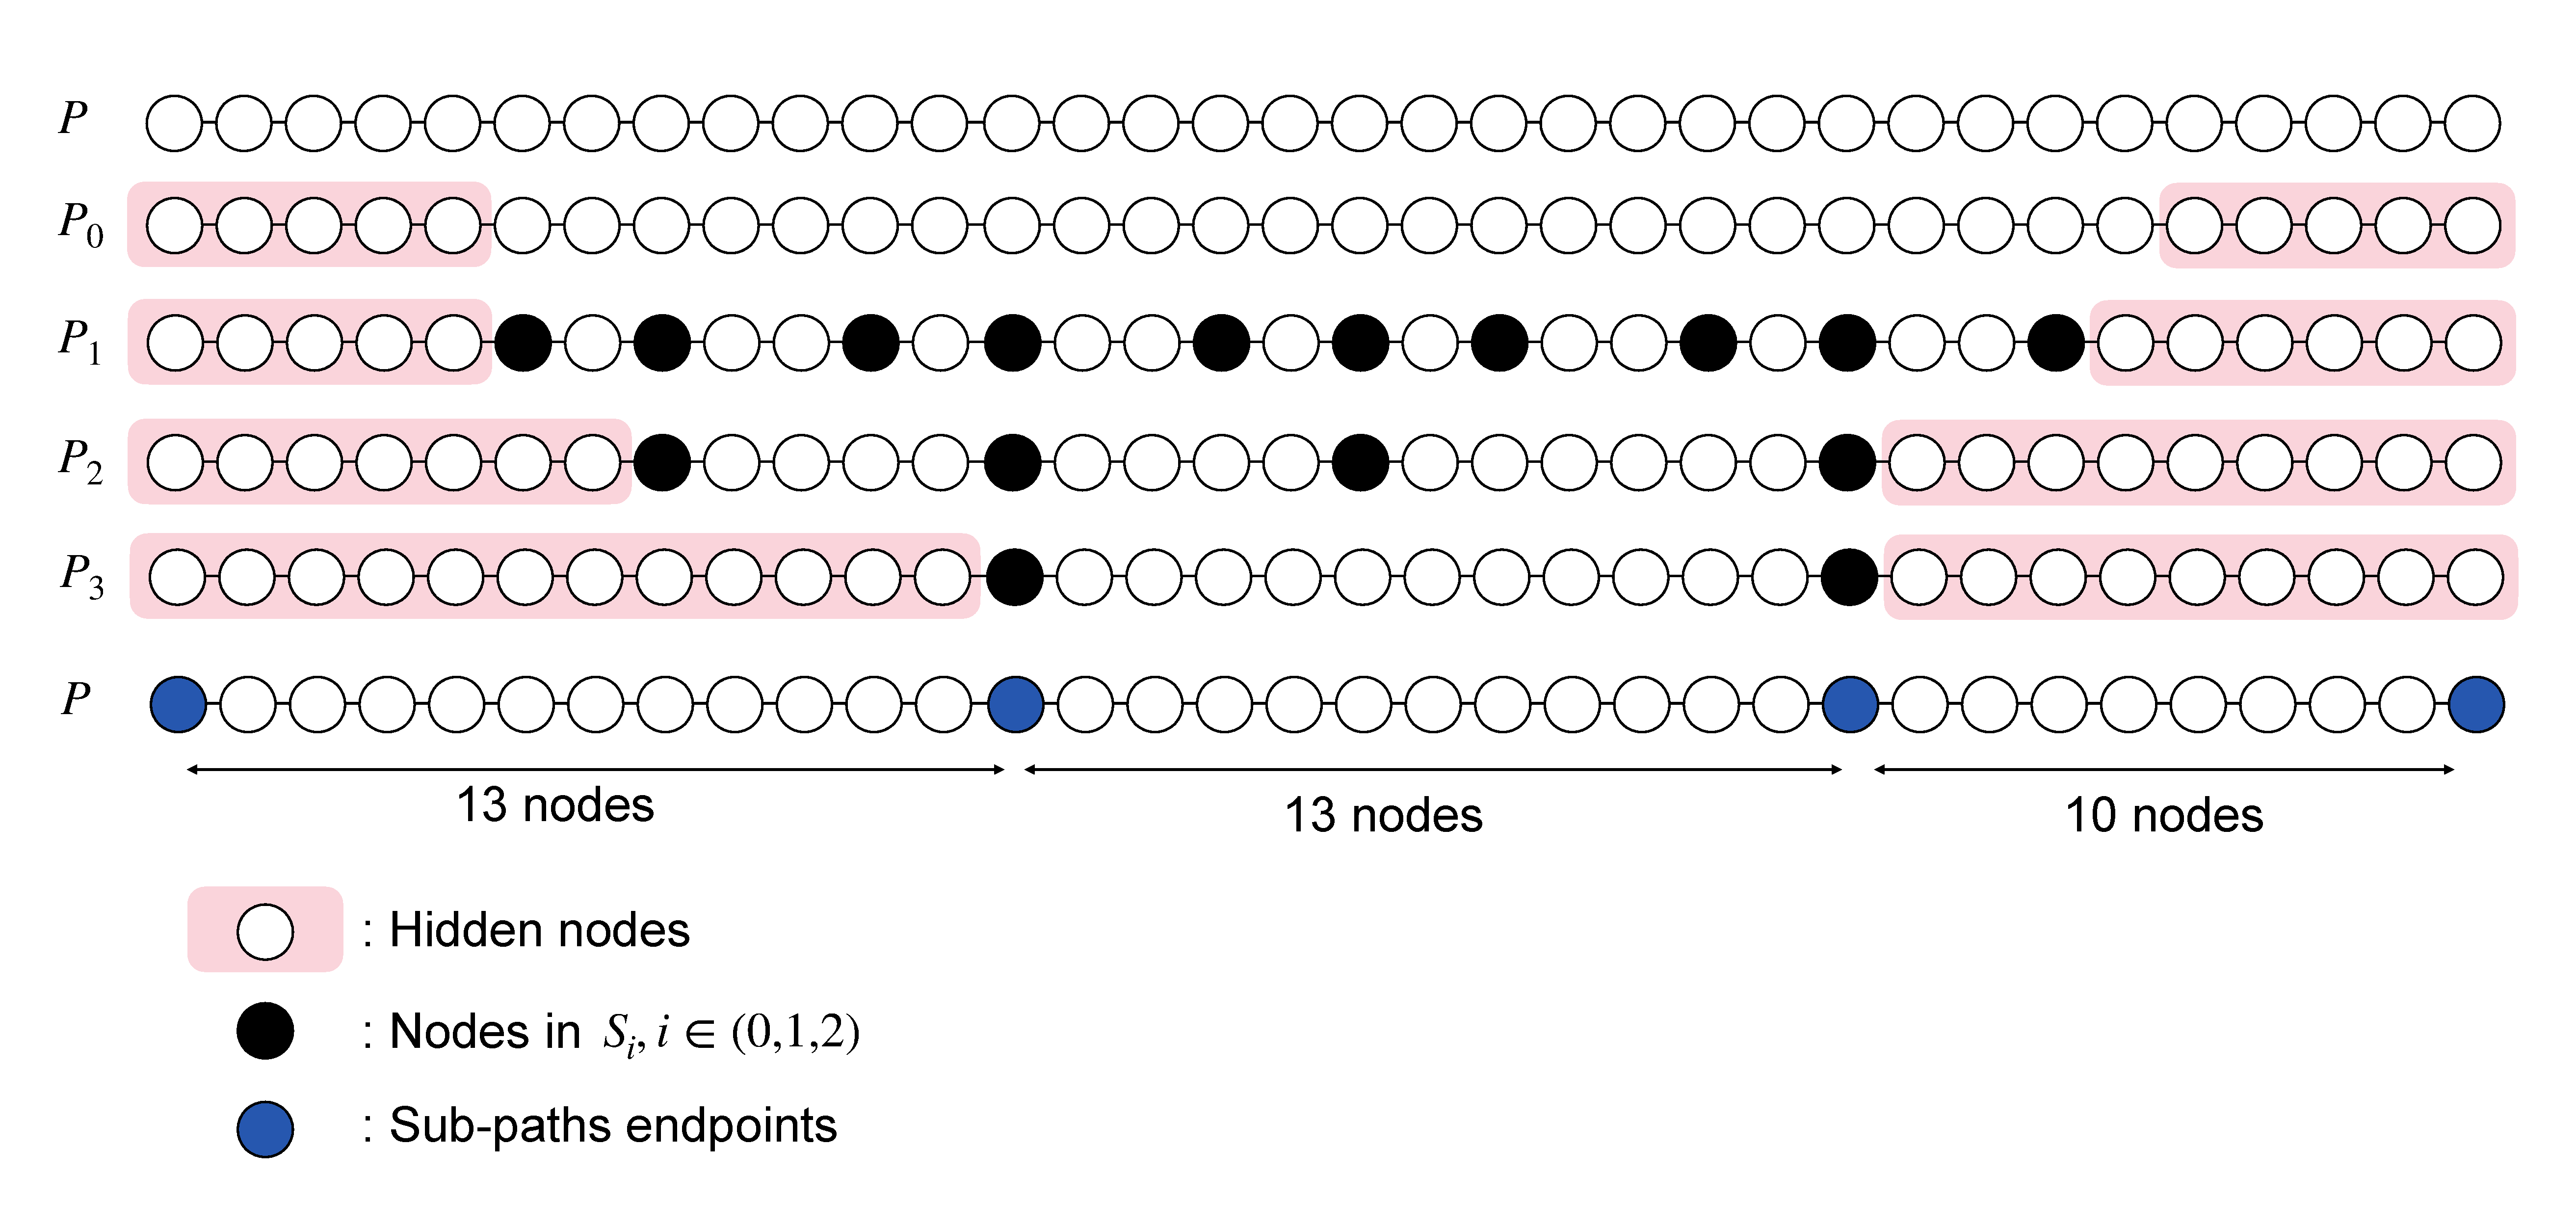
\includegraphics[scale = 0.20]{Figures/path.pdf}
    \caption{Execution of the splitting algorithm on a path}
    \label{fig:path}
\end{figure}
\end{proof}
\end{claim}
We now present a generic algorithm that, using the $RCP$ decomposition, labels all the edges of a graph $G'=(V',E')$ according to the constraints of a problem $\Pi=(3,2,W,B) \in \{\Pi_0\}\cup S_1\cup S_2\cup S_3$. Please note that it implies $B=\{AB,CC\}$.

We first apply the procedure $RCP(22)$ on $G$ and obtain the decomposition $V_1,V_2,...V_L$. We now process the layers from L to 1.
For each node from a layer $V_i$, it can either be a degree-1 node, either part of a long path
\begin{itemize}

    \item \textbf{Step 1}
    We first label the edges of the \textit{white} nodes that are in low-degree$(G_{i-1},1,1)$, there are 2 possibilities depending on $v$, the neighbor of $u$ that is in a layer $V_j$ with $j \in \{i,i+1...,L\}$.
    \begin{itemize}
        \item $v \in V_u$ with $u \in \{i+1,...,L\}$
        
        In this case, since $u$ has only one edge already labelled, it should always be possible for it to label its 2 other edges with respect to the $W$ configurations set since it is not empty.
        
        \item $v \in V_i$
        
        In this case, $v$ is on the same layer as $u$, however, since $v$ is a black node according to the proper coloring of the graph, it should not yet have colored any of its edges and does not have any neighbor from a higher layer. Hence $u$ can safely label all its edges with any configuration.
    \end{itemize}
    
    \item \textbf{Step 2}
    We now label the edges of the \textit{black} nodes that are in low-degree $(G_{i-1},1,1)$, from what have been done in step 1, a black node $u$ will always have exactly one of its edges already labelled, it can then label its other edge according to $B$ since it is not empty.
    
    \item \textbf{Step 3}
    Note that this step can be applied to all long paths of the layer in parallel since all of them are different connected components. Considering that the same process applies to all of them, we will detail what is done to one of them. Note that the running time is not influenced as it is done in parallel.
    
    \textbf{Step 3.1 : Redefining the endpoints of the path}
    
    Now that all degree-1 nodes of the layer have been labelled, we will try to label all black and white nodes that are in a long path that starts from a node $u_1$ and goes to a node $u_2$. We first look at the color of the two endpoints $u_1$ and $u_2$. For each of them, we do the following : let $u_x$ be one of them:
    \begin{itemize}
        \item If $u_x$ is black, it must have one edge $e_1$ that has already been labelled, its other edge $e_2$ can hence already be labelled ($e_1 = A \rightarrow e_2 = B, e_1= B \rightarrow e_2 = A, e_1 = C \rightarrow e_2 = C$)
        \item If $u_x$ is white, let be $e$ its edge that has already been labelled. Let's look at the neighbor of $u_x$ that is incident to $e$, it must be a black node for which both edges are already properly labelled. We then define it as the new endpoint of the path.
    \end{itemize}
    The above leads both of the endpoints of the path $P$ to be black nodes and the path to have now a minimal length of 23 nodes.
    
    \textbf{Step 3.2 : Splitting the path into chunks}
    
    \begin{defi} (Chunk of length n). A chunk of length n is a path of n nodes properly colored. Its two endpoints are \textit{black} (hence $n=2k+1$ for some $k\in \mathbb{N}$)
    \end{defi}
    
    We will now look at the path $P'$ that is the path $P$ where we use the the node-as-edge notation, as we define white nodes as edges. This leads $|P'|\geq 12$.
    Using the claim \ref{claim:path}, we will now split this path into at least 2 chunks of length $\geq 6$ in time $\mathcal{O}(\log^*n)$ where each chunk shares at most $1$ black node (common endpoint).
    
    If 2 chunks are adjacent and hence share a black endpoint $u$, we label both of $u$'s incident edges with C, since $CC$ must be in $B$, this is correct.
    
\item \textbf{Step 4}

In this step, we show how to label all the nodes of a chunk $Y$ with $|Y|\geq 11$, note that again, the labelling of the chunk can be done in parallel on every chunk. Since a chunk must have a length of at most $28$ black nodes according to the claim \ref{claim:path}, such a labelling is done in constant time since $|Y|\leq 55 = \mathcal{O}(1)$.

\begin{defi}
    (Chunk labelling). Given a problem $\Pi=(3,2,W,B)$ a chunk labelling $P(n_{min})$ is a regular expression using the labels of $\Sigma$ such that for every $n>=n_{min}$ with $n=2k$ for some $k\in\mathbb{N}$, it represent a unique string of length n respecting the following: for $i\in\{0,...,n-2\}$
    \begin{itemize}
        \item If $i=2k$ for some $k\in\mathbb{N}$: we have $(P_{i}P_{i+1}X)\in W$ for some $X\in \Sigma$
        \item If $i=2k+1$ for some $k\in\mathbb{N}$ we have $(P_{i}P_{i+1})\in B$
    \end{itemize}
    \end{defi}
\begin{claim}
\textit{Given a chunk labelling $P(n_{min})$ it is possible to label the edges of a chunk of length $n>=n_{min}+1$ in time $\mathcal{O}(n)$ according to a black and a white constraint B and W}
\begin{proof}
Let be the chunk as follow :
\begin{itemize}
    \item $V=\{v_i$ for $i\in\{0,...,n-1\}\}$
    \item $E=\{(v_i,v_{i+1})$ for $i\in\{0,...,n-2\}$
    \item $v_i$ is black if and only if $i=2k$ for some $k\in\mathbb{N}$ 
\end{itemize}
We are given a chunk labelling $P$, we label each edge $e = (v_i,v_{i+1})$ for $i\in\{0,...,n-1\}$ with $P[i]$.

Let's now take a black node $v_i$ and show that it must be properly labelled. Because $v_i$ is black, $i=2k$ for some $k\in\mathbb{N}$ its 2 incident edges have been labelled with respectively $P[i-1]$ and $P[i]$. By definition of the chunk labelling, $P[i-1]P[i]\in B$ since $i-1$ is odd.

We now show in a similar way that a white node $v_j$ must also be properly labelled. Because $v_j$ is white, $j=2k+1$ for some $k\in\mathbb{N}$ its 2 incident edges have been labelled with respectively $P[j-1]$ and $P[j]$. By definition of the chunk labelling, there is a configuration $P[j-1]P[j]X\in w$ for some $X\in \Sigma$ since $i-1$ is odd.
\end{proof}
\end{claim}
\end{itemize}
Since there is at least 2 chunks per long path, we know for sure that the following must hold for any chunk $Y$ as shown in Figure \ref{fig:global_1}:
    \begin{itemize}
        \item One endpoint of $Y$ is a black node that has labelled its incident edge with $C$.
        \item The other endpoint is a black node that has labelled its incident edge to the chunk with any label. 
    \end{itemize}
    We also know that each chunk is composed of at least 6 and at most $28$ black nodes, including the 2 endpoints that have already labelled their incident edges.
    A chunk consists hence of at least 10 edges, so for each problem, we need to find the following chunk labellings:
\begin{figure}[htb]
    \centering
    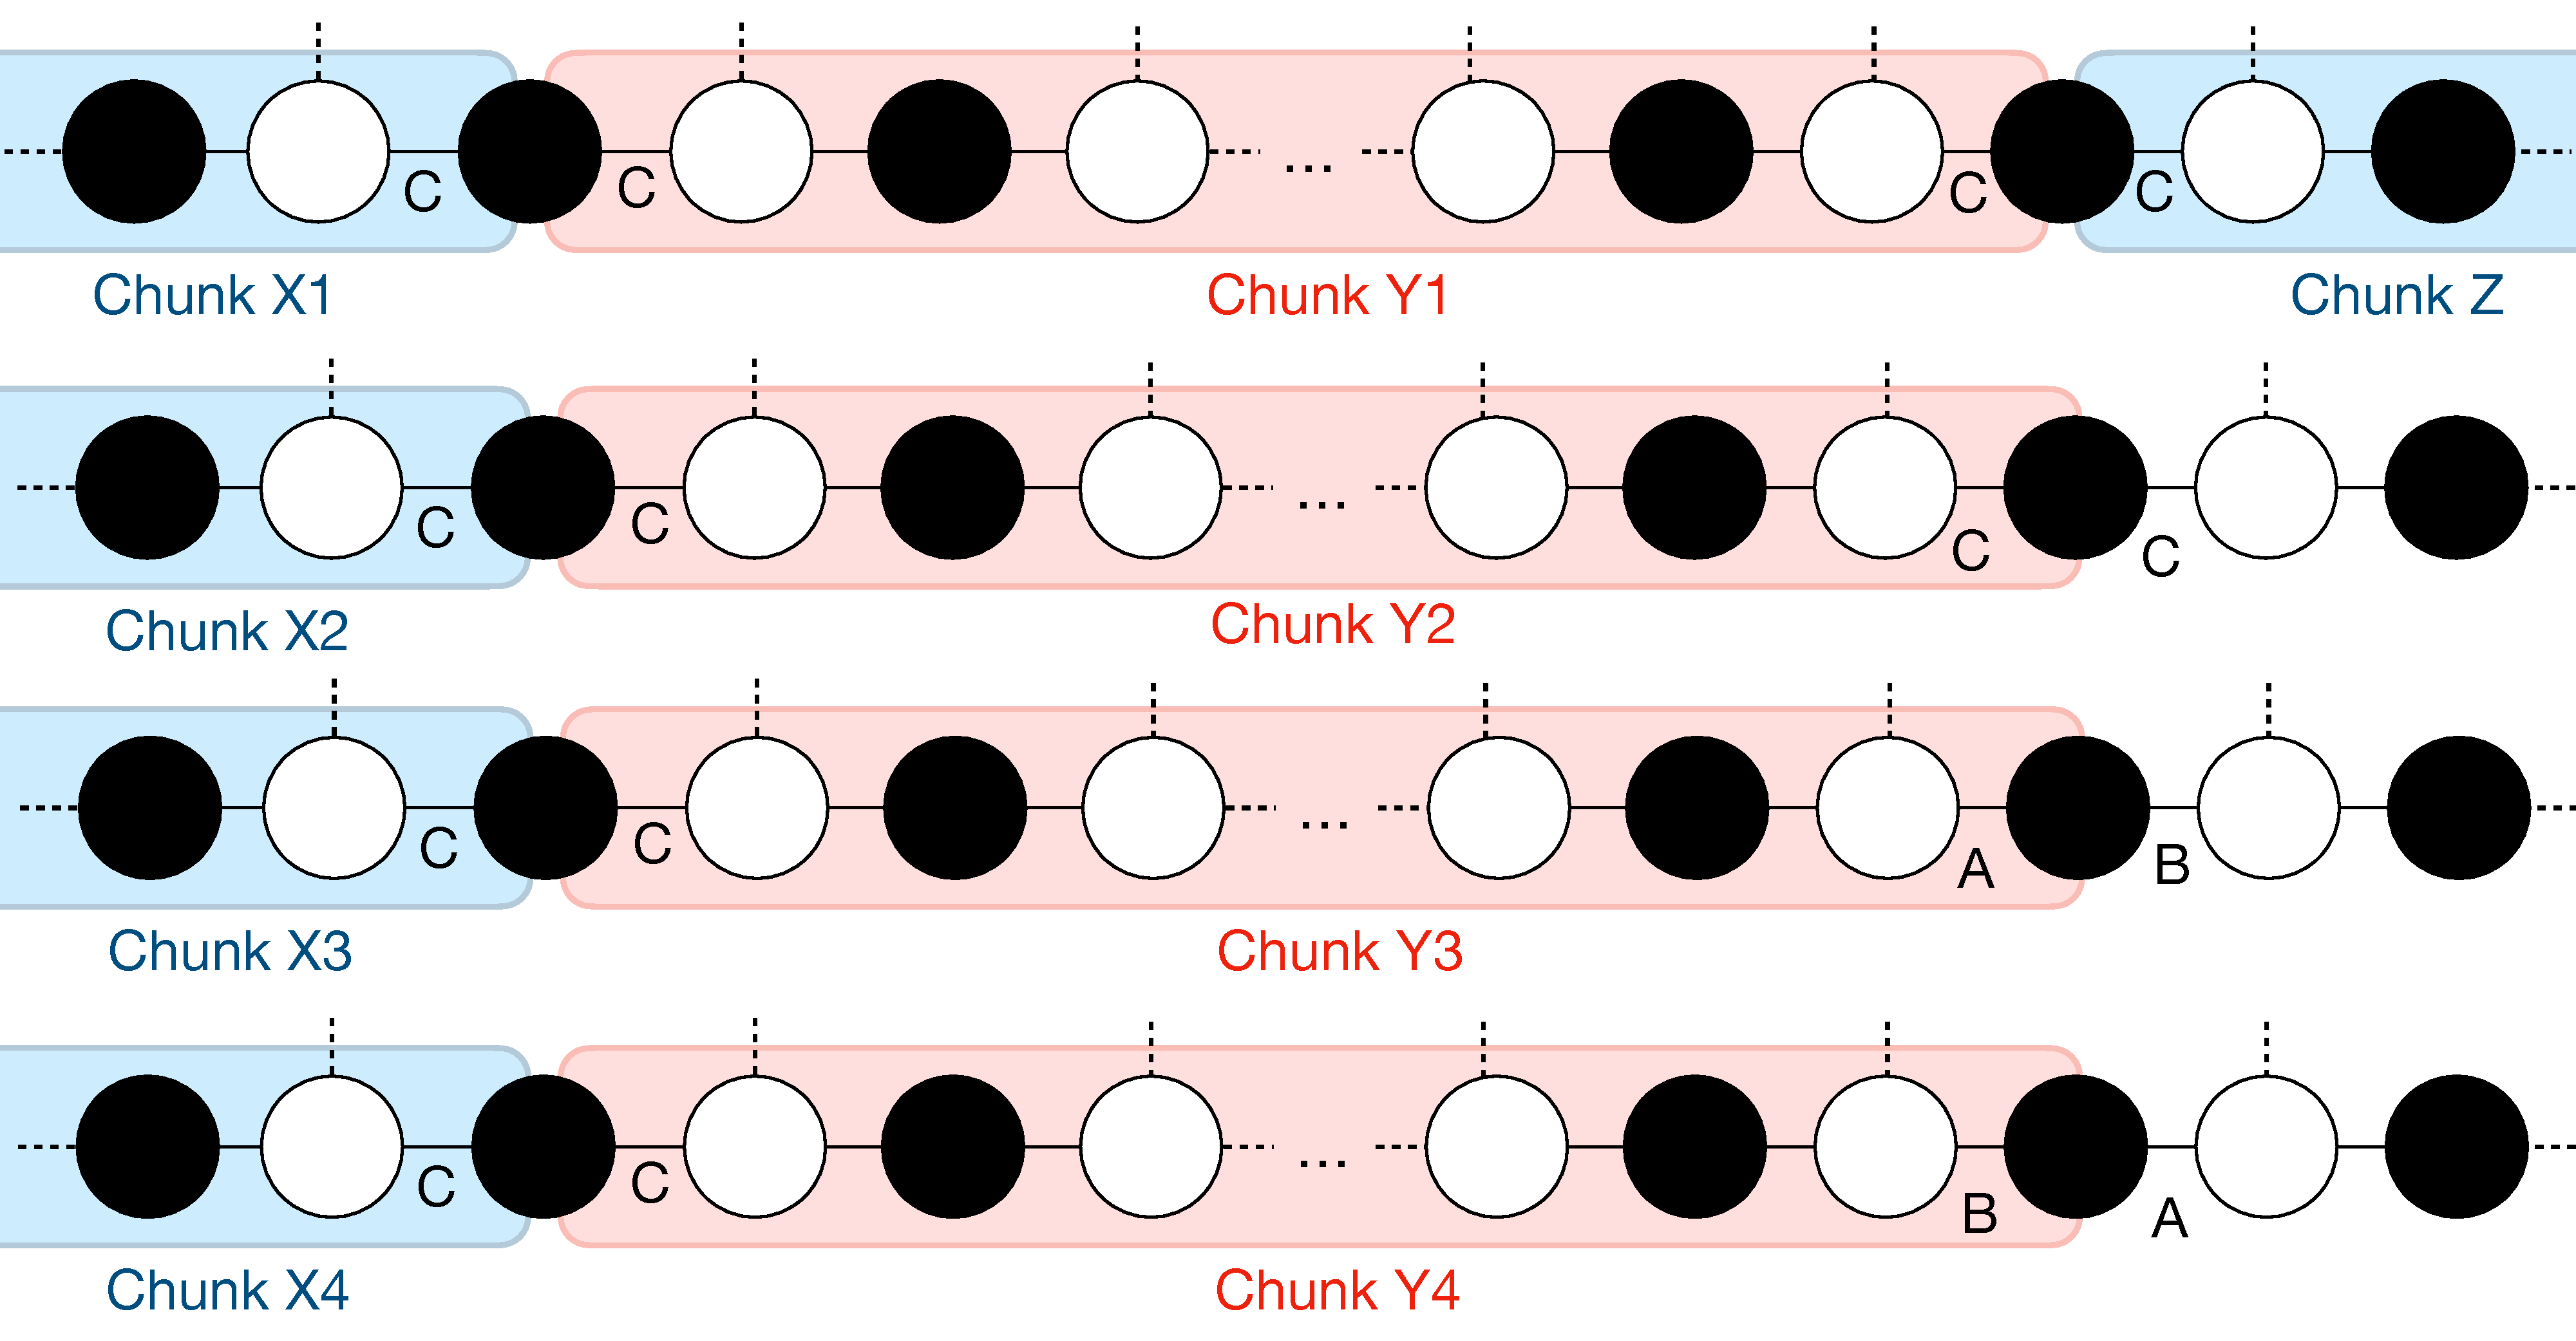
\includegraphics[scale = 0.22]{Figures/rcp_explain.pdf}
    \caption{The different chunk's endpoints possibilities}
    \label{fig:global_1}
\end{figure}
\begin{itemize}
    \item a) A chunk labelling $P_0(10)$ that starts with $C$ and ends with $C$ (Chunk Y1 and Y2 of Figure \ref{fig:global_1})
    \item b) A chunk labelling $P_1(10)$ that starts with $C$ and ends with $A$ (Chunk Y3 of Figure \ref{fig:global_1})
    \item c) A chunk labelling $P_2(10)$ that starts with $C$ and ends with $B$ (Chunk Y4 of Figure \ref{fig:global_1})
\end{itemize}

Table \ref{table:chunks} shows these 3 chunks labelling for each of the problems such that the left endpoint is always labelled with $C$.
We can now label the edges of each chunks in parallel in constant time since the length of each chunk is $\mathcal{O}(1)$.
\begin{table}
\centering
\small
\caption{Chunk labelling for each problem}\label{table:chunks}
\begin{tabular}{r|c|c|c}
    $\textbf{W}$ & $CC$ $(P_0(10))$ & $CA$ $(P_1(10))$ & $CB$ $(P_2(10))$\\
    \hline
    $\Pi_0 \rightarrow \{ABC\}$ & $\textbf{C}(AB)^k\textbf{C}$ & $\textbf{C}(AB)^k\textbf{A}$ & $\textbf{C}(BA)^k\textbf{B}$ \\
    \hline
    $S_1 \rightarrow \{ACC, BXC\}$ & $\textbf{C}(CC)^k\textbf{C}$ & $\textbf{C}(CC)^k\textbf{A}$ & $\textbf{C}(CC)^k\textbf{B}$\\
    \hline
    $S_2\rightarrow \{AAX,BCC\}$ & $\textbf{C}(CC)^k\textbf{C}$ & $\textbf{C}(CC)^q(CCBA)^k\textbf{A}$ & $\textbf{C}(CC)^k\textbf{B}$\\
    \hline
    $S_{3_a}\rightarrow \{AAA,BBC\}$ & $\textbf{C}(BAABCC)^q(BAAB)^k\textbf{C}$ & \multirow{3}{*}{$\textbf{C}(BA)^k\textbf{A}$} & \multirow{3}{*}{$\textbf{C}(BAAB)^k(CC)^q \textbf{B}$}\\
    $S_{3_b}\rightarrow \{AAB,BBC\}$ & $\textbf{C}(BAAB)^{k}(AB)^q \textbf{C}$ & &\\
    $S_{3_c}\rightarrow \{AAC,BBC\}$ & $\textbf{C}(BAAB)^k(BA)^q\textbf{C}$ & &
\end{tabular}
\newline\newline
with $X\in \{A,B,C\}, k\geq 1, q \in \{0,1\}$
\end{table}\\\\
We can hence iterate over the layers and label every node in it in a correct way, we can then solve problems described in time $\mathcal{O}(\log(n))$.



\section{Logarithmic lower bound}
\subsection{Using the round elimination}
We know that when using the round elimination \cite{round-eliminator}, finding a fixed point in a speed up on a problem $\Pi$ results in $\Pi$ having a $\Omega(\log(n))$ lower bound on its complexity. Unfortunately, the round eliminator does not include an automatic detection of such fixed points. However, we ran the auto lower bound tool with $iterations = 16$ and $labels = 5$. Whenever the round eliminator would return a lower bound of 17 rounds, it was very likely that it was a fixed point. Thus, it was manually checked.
\subsection{Results}
The above method was used on problems not yet classified having a white degree 3 and a black degree 2, leading the following ones (and then all their restrictions) to have a $\log(n)$ lower bound:\\
$$\begin{array}{ll}
    W =\{AAB,ABC,ABB\} & B = \{AC, BB, CC, AA, BC\}\\
    W = \{AAA,BBC,BBB,ABB\} & B = \{AC, AB, CC, BC\}\\
    W = \{BCC,BBC,AAC,AAB\}& B = \{BB, CC, AA\}\\
    W = \{BCC,AAC,ABB\} & B = \{BB, CC, AA\}\\
    W = \{BBC,AAB,BBB,AAC,BCC\}& B = \{CC, BC, AA\}\\
    W = \{ABB,AAA,BBB,BCC,ACC\}& B = \{AB, CC\}\\
    W = \{AAB,AAA,BBB,BCC,AAC\}& B = \{AB, CC\}\\
    W = \{AAC,BBC,BBB,ABB\}& B = \{AB, CC\}\\
    W = \{BCC,AAC,ABB\}& B = \{AB, CC\}\\
    W = \{BCC,AAA,ABC\}& B = \{AB, CC\}\\
    W = \{BBC,AAA,ABC\}& B = \{AB, CC\}\\
    W = \{BCC,BBC,AAA\}& B = \{AB, CC\}\\
    W = \{AAA,BBB,ABC\}& B = \{AB, CC\}\\
    W = \{BCC,BBC,AAA,ABC\}& B = \{AB, CC\}
\end{array}$$

\section{Results}
These lower and upper bounds, in the case where $\wdd = 3$ and $\bdd = 2$, led to the following: 990 classified problems as logarithmic and 16 unclassified problems left that can potentially have a global complexity.